\section{Resultados e Discussões}
\label{sec:resultados}
Considerando as abordagens desenvolvidas, torna-se necessária a realização de uma avaliação sistemática, com o objetivo de verificar se a abordagem evoluída resulta em melhorias e apresenta desempenho superior à abordagem inicial. Sendo assim, para avaliar a evolução do módulo de contagem de pessoas, foi realizada uma coleta de dados com o objetivo de analisar seu desempenho em comparação à abordagem anteriormente empregada e validar sua viabilidade de implementação. Para esse estudo, utilizou-se o conjunto de eventos presentes na Tabela \ref{tab:events_description}, o qual foi executado integralmente e por duas vezes consecutivas pelo autor deste trabalho, gerando um total de 16 rodadas para análise. Novos dados foram coletados, tendo em vista que mudanças físicas foram aplicadas ao sistema, logo a reutilização dos dados apresentados na etapa de análise exploratória não é interessante para a avaliação. 

O estudo realizado consistiu na implementação das duas abordagens aqui apresentadas — inicial e evoluída — em um ambiente virtual, com o objetivo de avaliar seu desempenho na caracterização do evento registrado em cada rodada. Para essa finalidade, utilizou-se a linguagem Python, por meio de Jupyter Notebooks, na construção de todo o fluxo de pré-processamento e análise previamente descrito na Subseção \ref{subsec:module_evolution}. Adicionalmente, as funções responsáveis por essas etapas foram desenvolvidas com o auxílio de bibliotecas amplamente empregadas em análise de dados, como NumPy, Pandas, SciPy e Matplotlib.

A Figura \ref{fig:heatmap_results} apresenta os resultados obtidos durante o processo de caracterização de eventos de interesse para as duas abordagens avaliadas. O gráfico consiste em um mapa de calor categórico que representa as duas execuções do estudo, suas respectivas rodadas e o resultado da caracterização do evento, sucesso ou fracasso. A partir da análise visual, observam-se dois padrões principais: (i) a dificuldade da abordagem inicial em caracterizar os eventos das rodadas 1, 2 e 8, atribuída a uma peculiaridade inerente à própria estratégia; e (ii) o fracasso de ambas as abordagens em identificar o evento da Rodada 2 durante a Execução 2, o que motivou uma análise detalhada desse conjunto de dados, revelando problemas na captura do evento que comprometeram sua correta caracterização.

\begin{figure}[H]
    \center
    \fbox{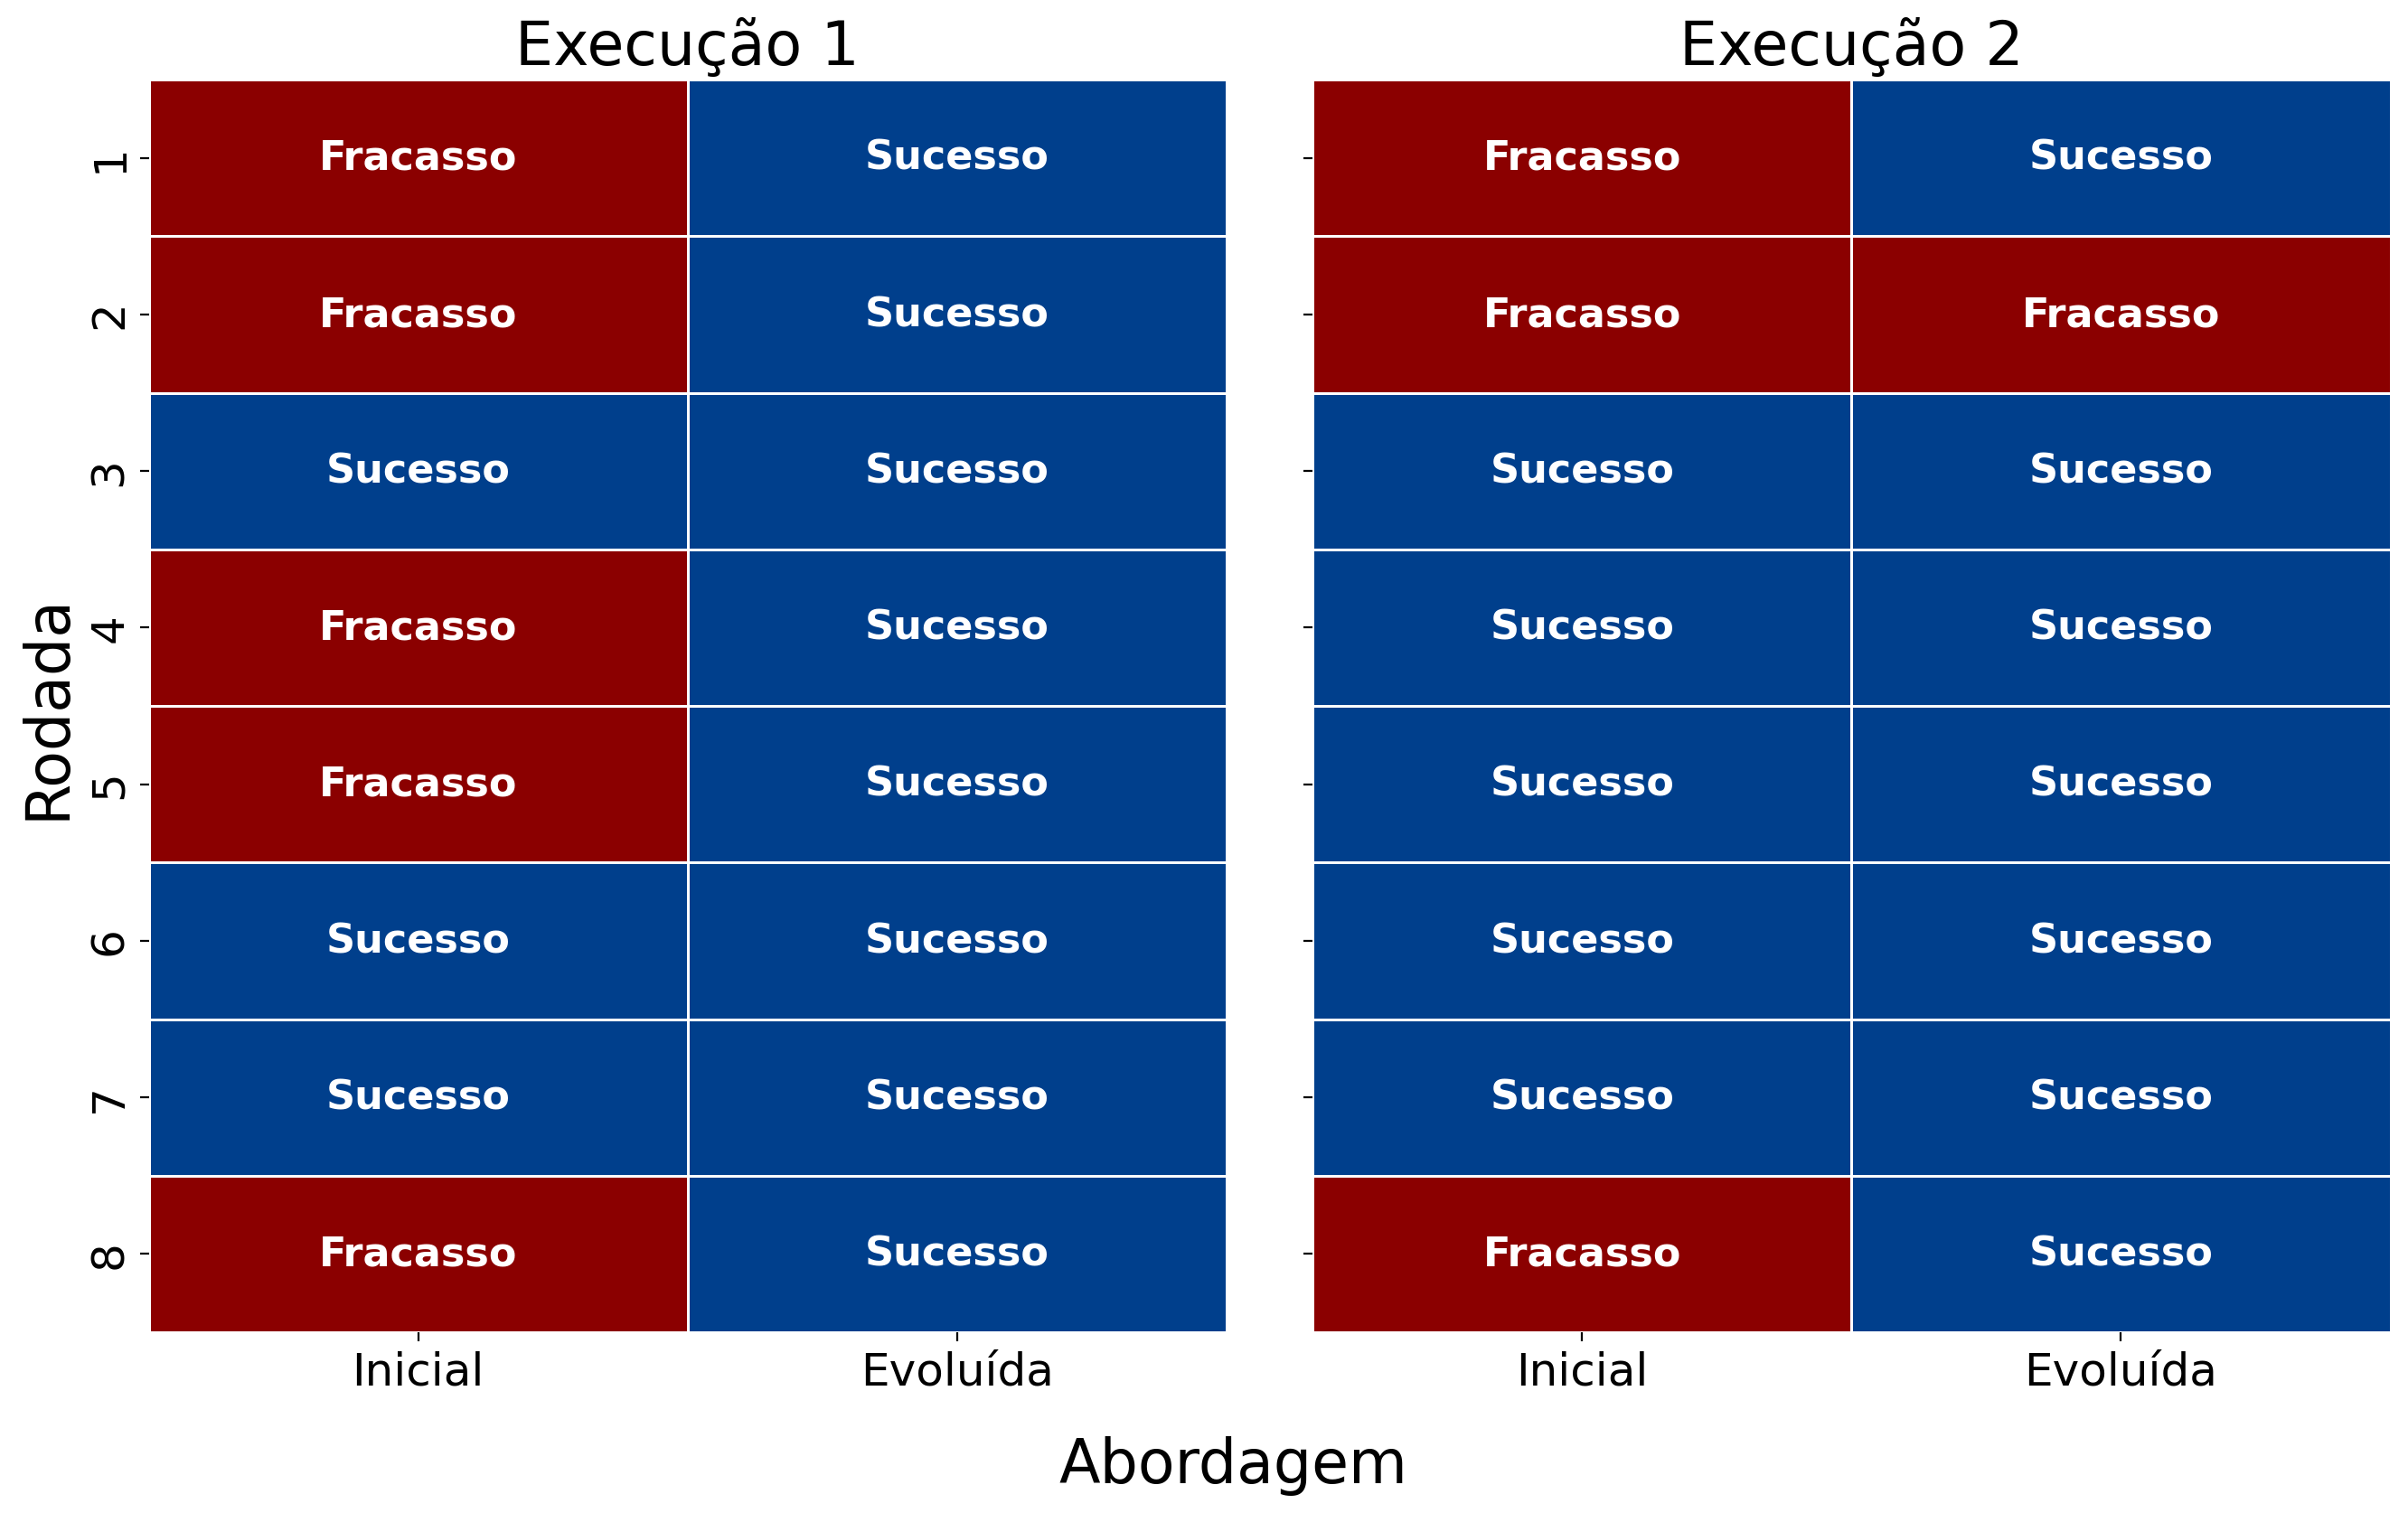
\includegraphics[scale=0.40]{images/heatmap_results.png}}
    \caption{Comparação entre as abordagens na identificação de eventos}
    \label{fig:heatmap_results}
\end{figure}

Ademais, observa-se que a abordagem evoluída apresenta resultados estáveis entre as execuções, obtendo sucesso em todas as rodadas, com exceção da Rodada 2 da segunda execução, cuja captura inadequada, conforme discutido anteriormente, limita análises mais conclusivas sobre esse caso específico. Esse padrão evidencia maior confiabilidade da abordagem evoluída em comparação à inicial, visto que seu desempenho permanece invariável para mesma rodada em diferentes execuções, ao passo que a estratégia inicial apresenta maior variabilidade e número de insucessos, como apresentado na Figura \ref{fig:bar_graph_results}.

\begin{figure}[H]
    \center
    \fbox{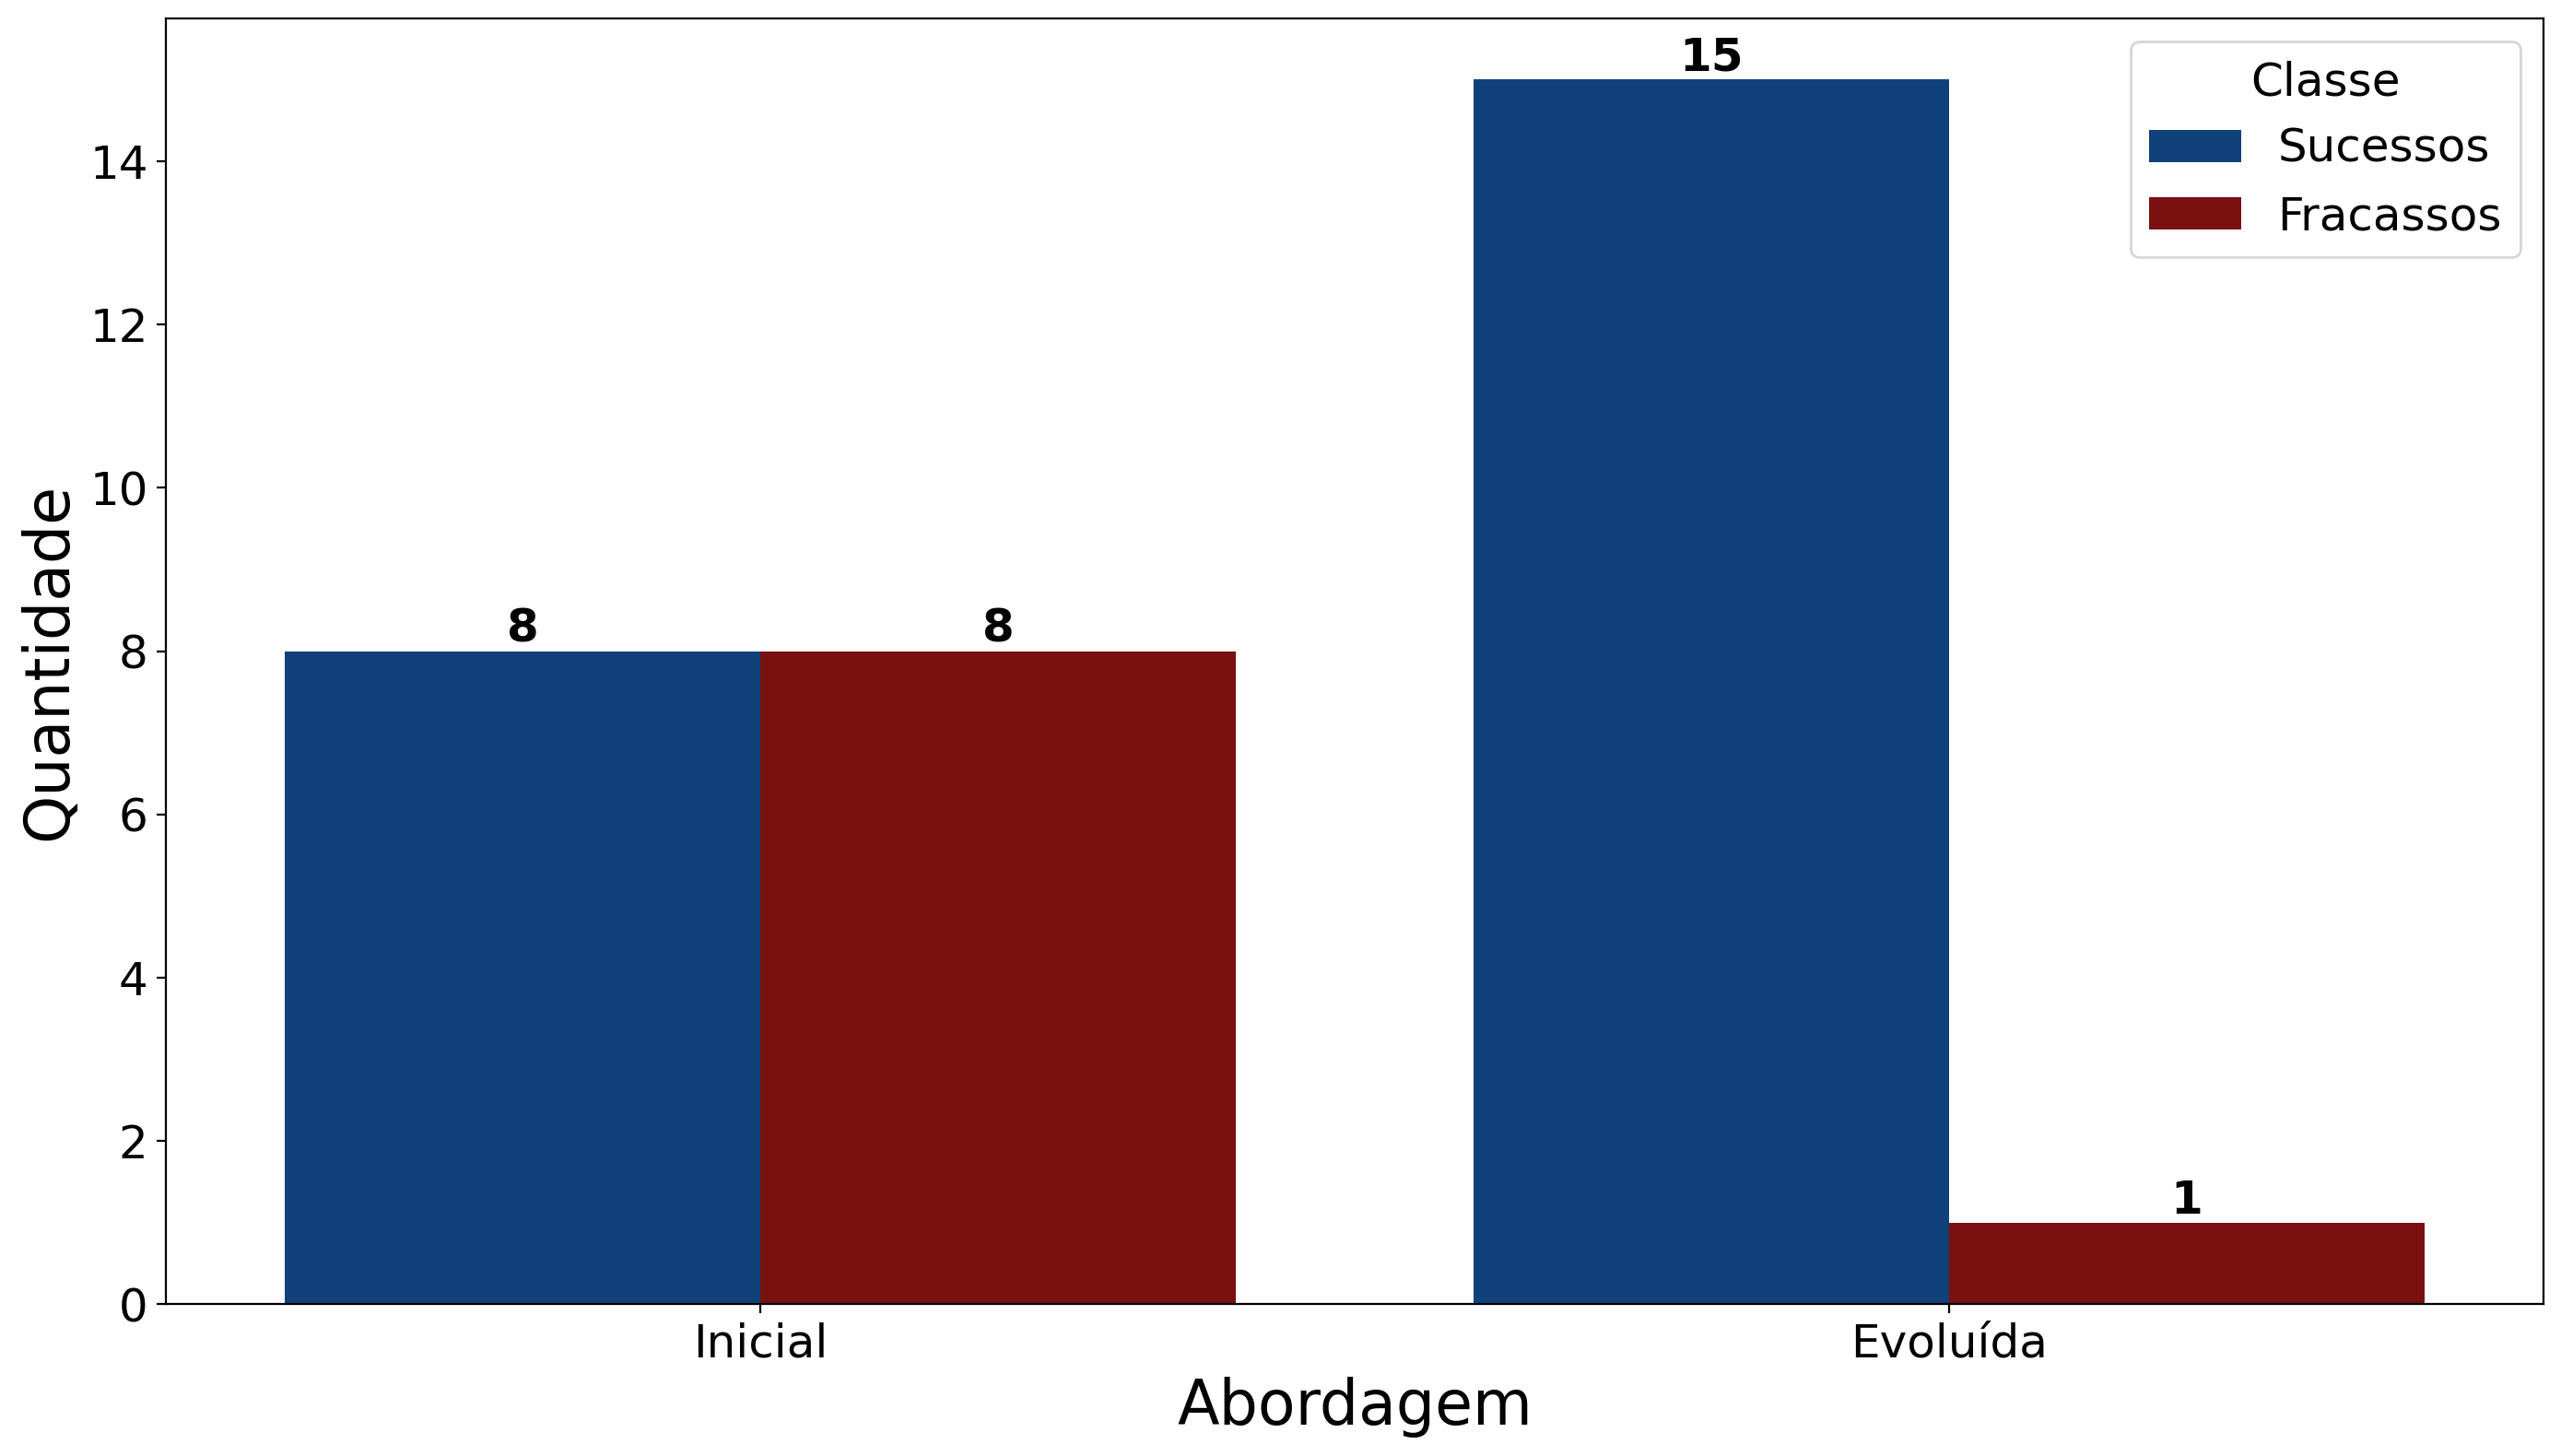
\includegraphics[scale=0.40]{images/bar_graph_results.png}}
    \caption{Comparação quantitativa entre as abordagens}
    \label{fig:bar_graph_results}
\end{figure}

Além de apresentar maior consistência, a abordagem evoluída também obteve taxa de sucesso superior na caracterização de eventos de interesse em relação à abordagem inicial, conforme ilustrado na Figura \ref{fig:bar_graph_results}. Das 16 rodadas avaliadas, o algoritmo evoluído falhou apenas uma vez, obtendo uma taxa de sucesso de $93{,}75\%$, enquanto a estratégia inicial apresentou 8 fracassos, representando uma porcentagem de sucesso de $50\%$ na avaliação dos mesmos conjuntos de dados. Por último, destaca-se que o único evento em que a abordagem evoluída obteve insucesso corresponde há uma rodada com problemas na captura dos dados, logo torna-se inconclusa a análise deste evento. 

Em virtude dos fatos descritos, compreende-se que o desempenho superior da abordagem evoluída em contraste a original, ocorre principalmente devido ao processo de suavização dos dados presente na estratégia. Como descrito na subseção de análise exploratória dos dados, a adoção dessa técnica mitiga o efeito de medidas incorretas e a interferência entre sensores, resultando em uma variação de estados de ativação dos sensores mais comportada e consequentemente a identificação correta do evento de interesse. Além disso, devido a adoção de etapas para detecção e construção de eventos de interesse, todos os conjuntos de dados analisados tendem a ter perfil semelhante, algo que impacta diretamente a consistência dos resultados. 

